% !TeX spellcheck = en_US
\chapter{Software architecture}

% http://jeffreypalermo.com/blog/the-onion-architecture-part-1/

Onion Architecture was used for overall design, this allows multiple frontends, so if the User Story 8 was to be developed, no refactoring would be required to the already existing business logic. The main namespaces can be seen in figure \vref{fig:Namespaces}, excluding testing namespaces.

Included in the Onion Architecture is the Repository Pattern, allowing for ao quick change from an in-memory database to an external if needed.

\begin{figure}
\centering
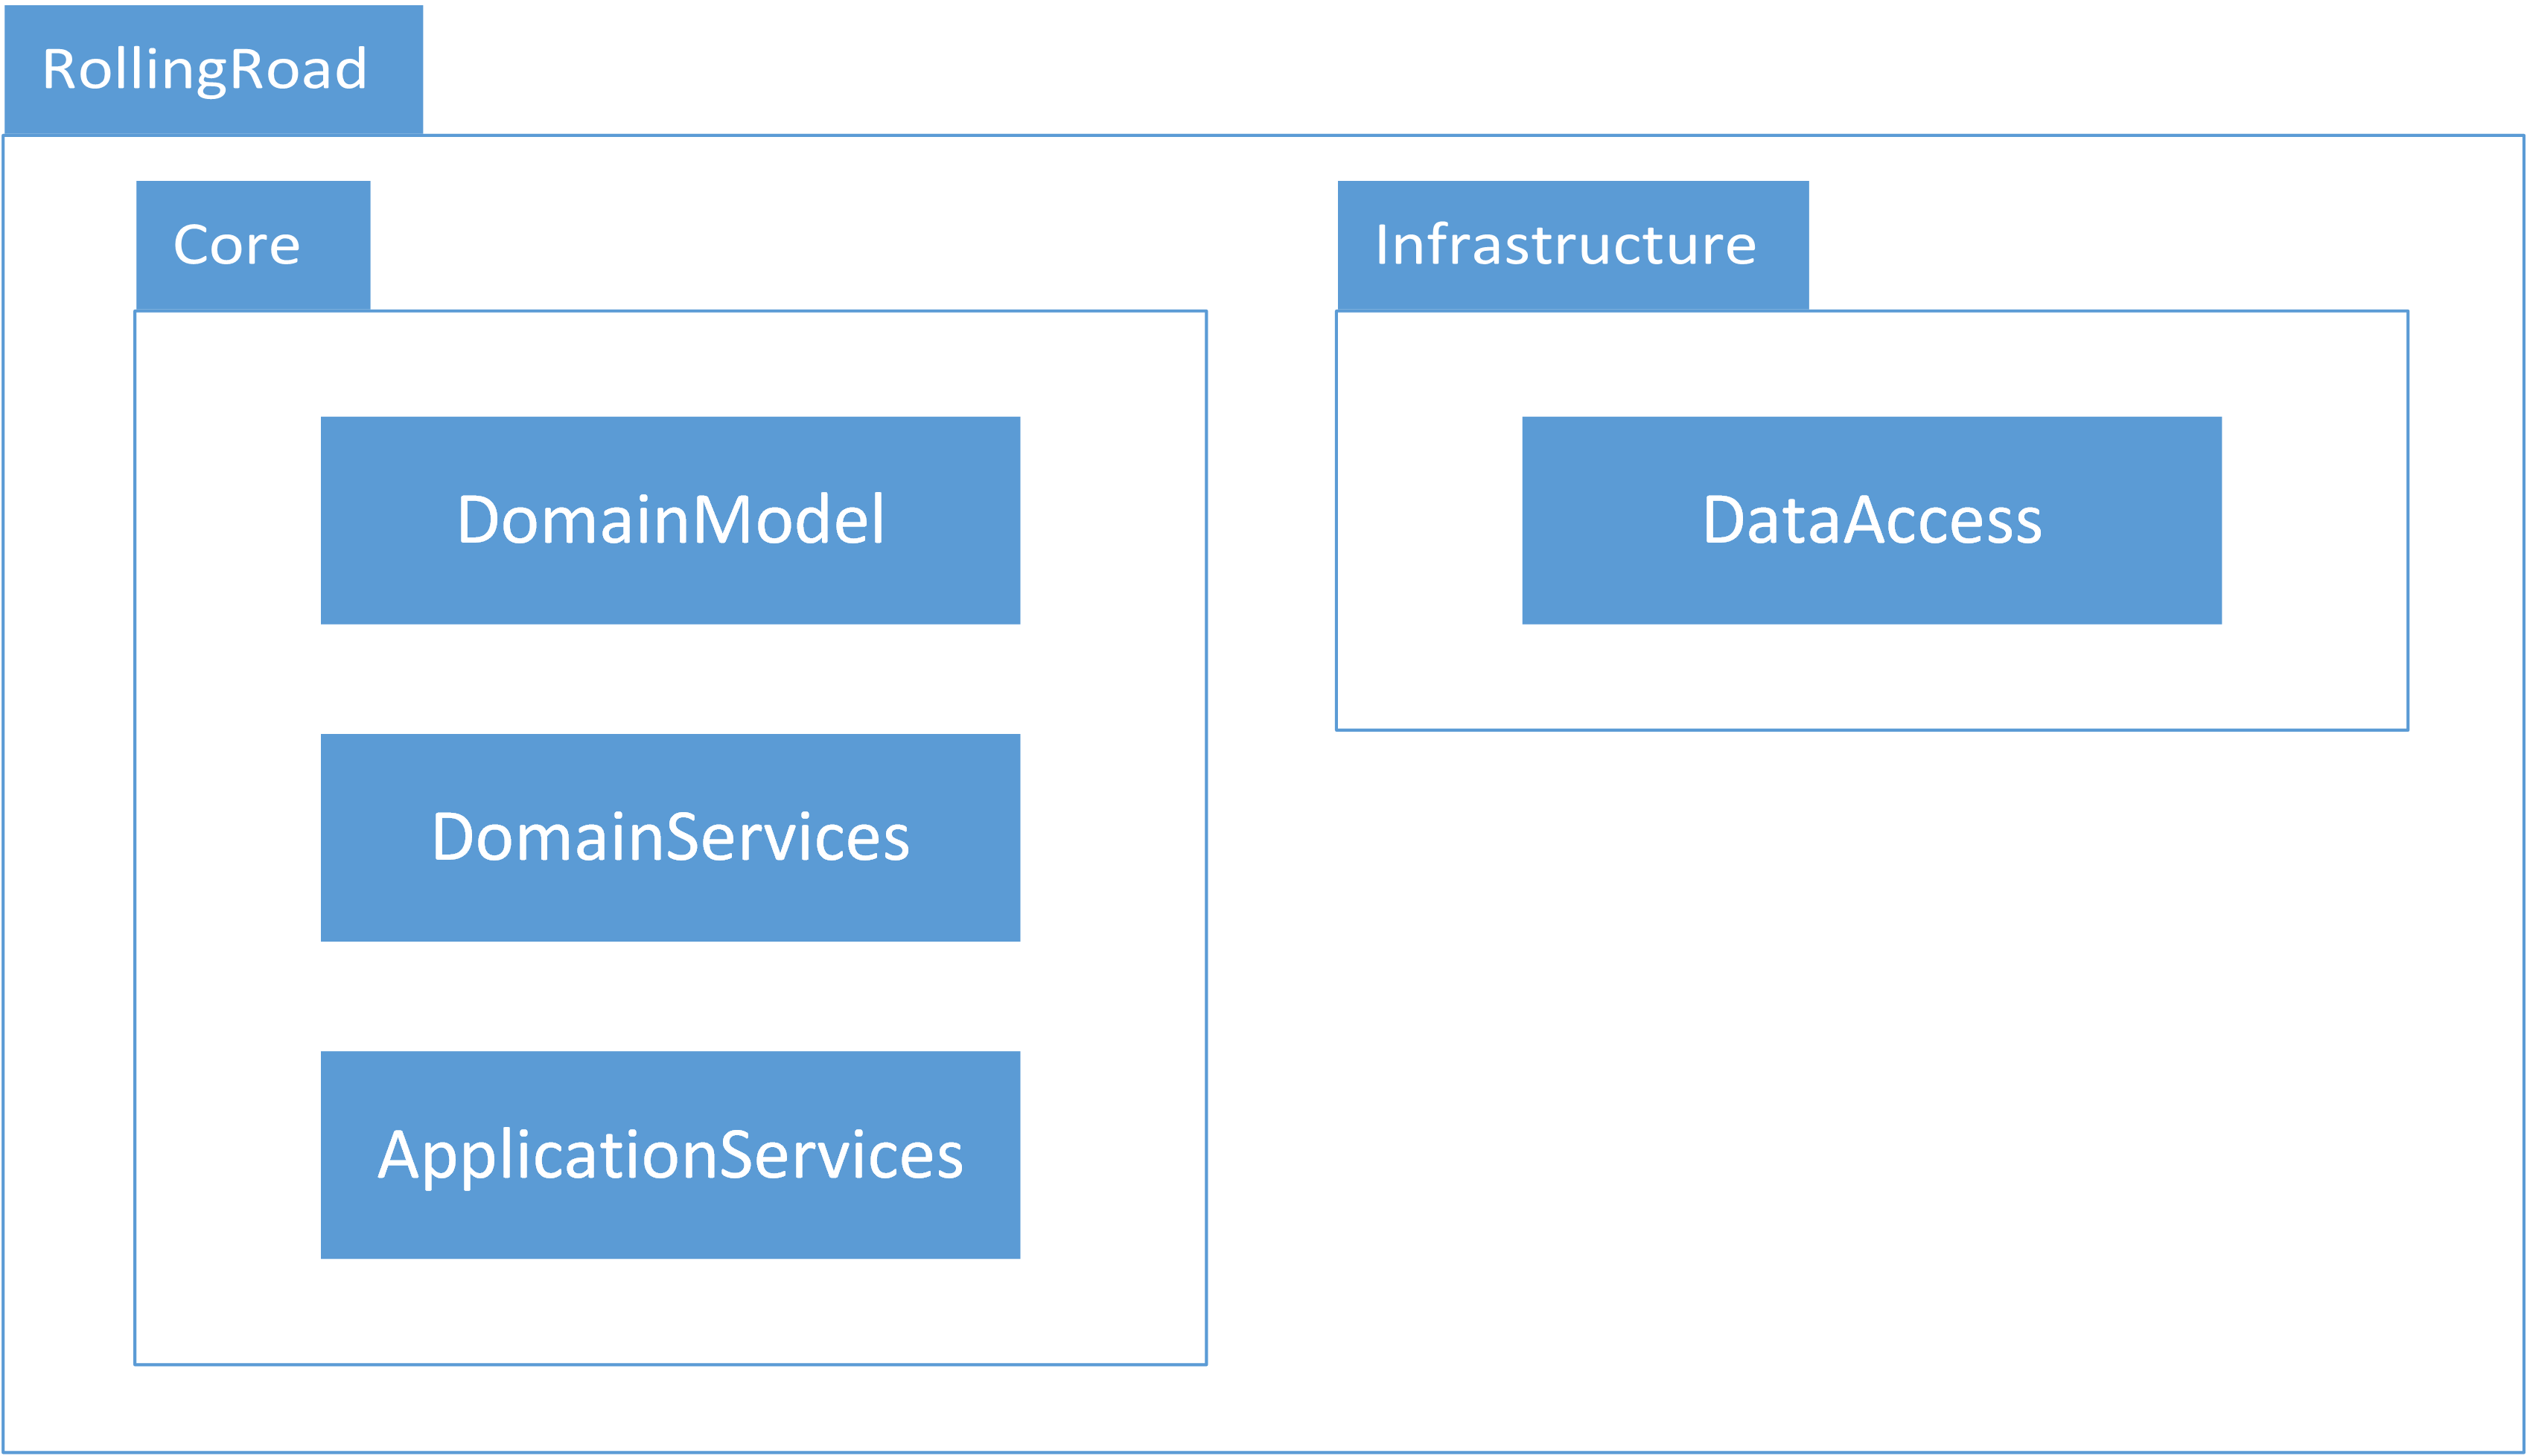
\includegraphics[width=0.7\linewidth]{Images/Namespaces}
\caption{Main namespaces}
\label{fig:Namespaces}
\end{figure}
